\chapter{Operating System}

\section{Introduction}

An operating system (\textbf{OS}) is the software that manages the computer hardware, creating some logical resources that other software and users can use. It's the logical support which controls and manages the physical components.

\begin{center}
    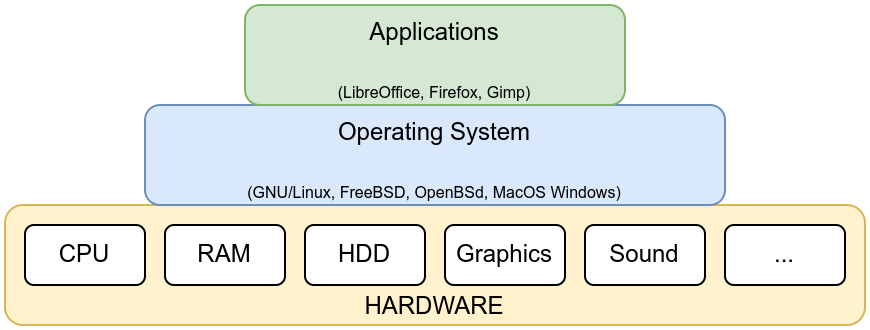
\includegraphics[width=0.9\linewidth]{operating_system.png}
\end{center}

Before the existence of operating systems, the hardware was available directly to the program, so every program must implement the access to the memory, the hard disk, how to read/write files...

\section{Software hierarchy}
The computer runs software, and this software can be classified:

\begin{itemize}
    \item \textbf{System's software}: Controls and manages the hardware of the computer. In this group: \textbf{operating systems}, \textbf{drivers} and \textbf{firmwares}.

    \item \textbf{Service programs}: Those are the networking services, system's services, and some services that the operating system uses. For example: networking management tools, disk partitioners, process manager ...

    \item \textbf{Utility programs}: The software that the end users use in order to do some basic stuff. Word processors, music utilities, games, ...
\end{itemize}

In this chapter we are going to focus on the system software, specifically the \textbf{operating system}.


\section{History of operating systems}
Let's see a brief history of operating systems.

\subsection{No operating systems (0-generation)}
The first computers were mainframes (big computers used by organizations), which didn't have any form of operating system.

The user which wanted to use the computer had to  schedule a period of time, because those computers hadn't got time sharing, only one program could run in each time.

First programs were coded in \textbf{machine code}, which is represented with '0' and '1', also called \textbf{binary code}.

Those programs had full access to the hardware, and because of that, every program had to implement access to those resources.

This period started with the digital computers until the late 1950s.

\begin{center}
    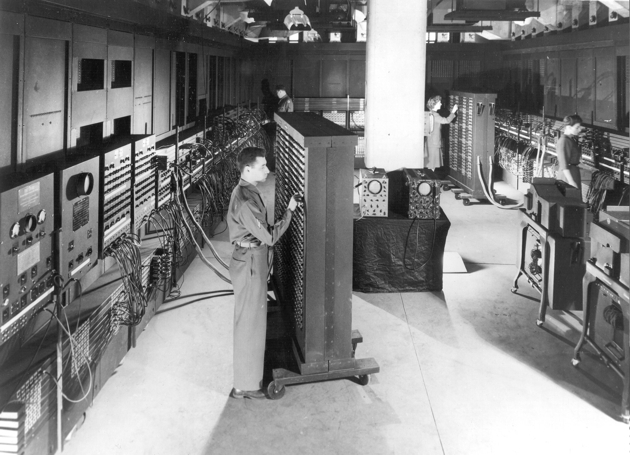
\includegraphics[width=0.6\linewidth]{ENIAC.jpg}
    \vspace{-10pt}\captionof{figure}{\href{https://en.wikipedia.org/wiki/ENIAC}{ENIAC computer. Source: Wikipedia}}\vspace{-13pt}
\end{center}


\subsection{Batch processing (1st generation)}
The computers became faster, and in order to no waste time, the \textit{\textbf{monitors}} were developed (the forerunners of operating systems). Those \textit{monitors} could process a series, or “batch”, of programs, often from magnetic tape.

\begin{center}
    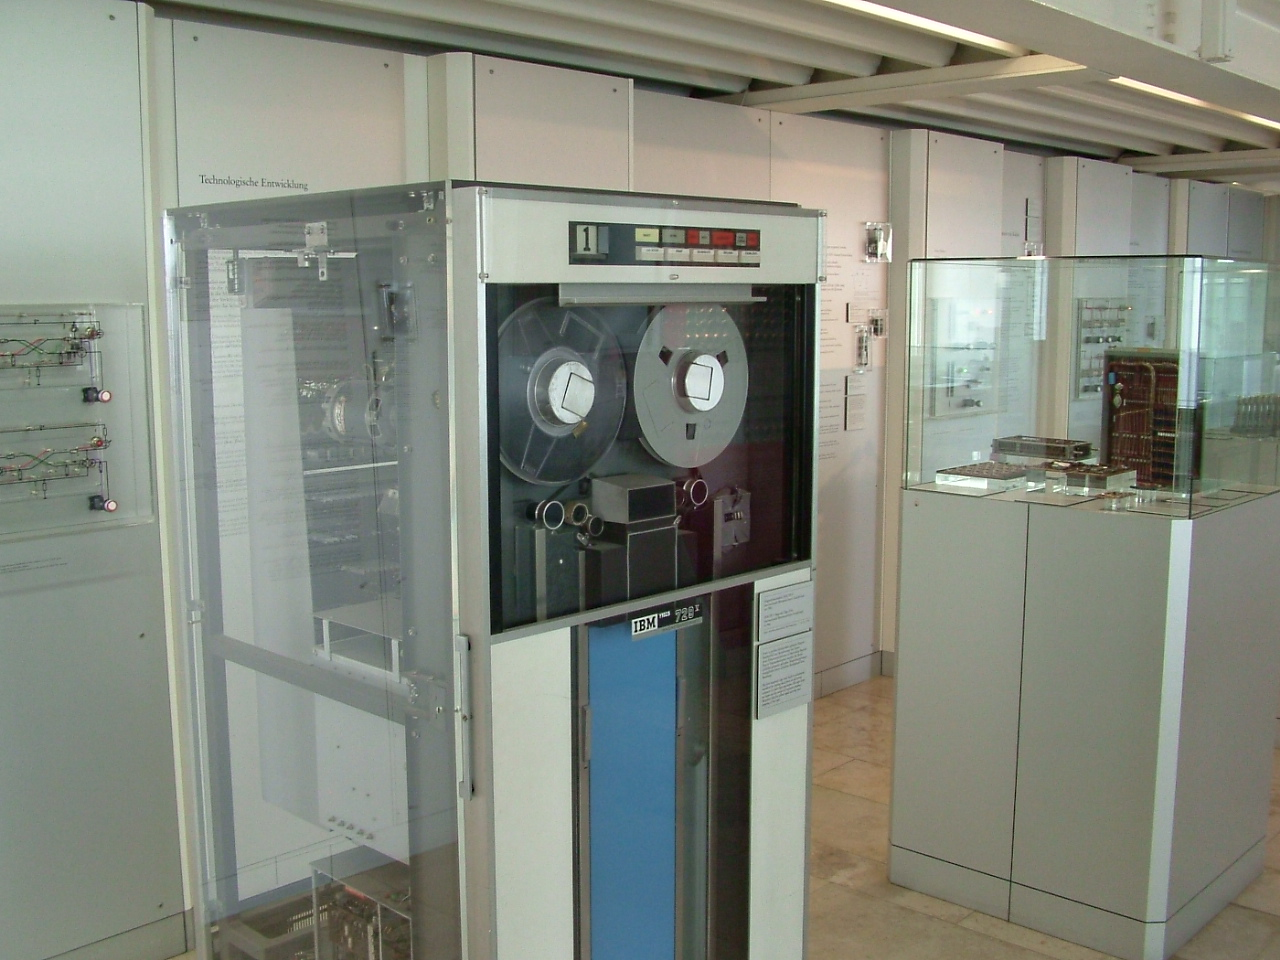
\includegraphics[width=0.6\linewidth]{tape.jpg}
    \vspace{-10pt}\captionof{figure}{\href{https://en.wikipedia.org/wiki/Magnetic-tape_data_storage}{Magnetic tape from IBM. Source: Wikipedia}}\vspace{-13pt}
\end{center}

The monitor would be loaded into the computer and run the first job of the batch. At the end of the job it would regain control and load and run the next until the batch was complete. The \textbf{output} of the batch would be written to magnetic tape or printed.


\subsection{Second generation}
In the 1960s, with the introduction ot the \href{https://en.wikipedia.org/wiki/Integrated_circuit}{integrated circuits}, the computers increased in speed, so the operating systems evolved trying to use this speed, using new techniques:

\begin{itemize}
    \item \textbf{Multiprogramming}: In any modern operating system there can be more than one instance of a program loaded in memory at the same time. For example, more than one user could be executing the same program, each user having separate copies of the program loaded into memory

    \item \textbf{Spooling}: Is a specialized form of multi-programming for the purpose of copying data between different devices. Was used to mediate access to punched card readers and punches, magnetic tape drives, and other slow, sequential I/O devices.

    \item \textbf{Buffering}:\textbf{Data buffer} (or just buffer) is a region of a memory used to temporarily store data while it is being moved from one place to another.
\end{itemize}

\subsection{Third generation}
With the evolution of computers, which began to allow the use of several processors, and more complex systems, operating systems evolved along with them. This generation is between 1965 and 1980.

\begin{itemize}
    \item \textbf{Multitasking}: Is the concurrent execution of multiple processes over a certain period of time. New tasks can interrupt already started ones before they finish, instead of waiting for them to end.

    When the computer has multiple processors, the multitasking is real, because each processor can execute one process at the same time.

    \begin{minipage}{0.6\linewidth}
        \item \textbf{Virtual memory}: Is a memory management technique that allows the use of the hard disk as part of the main memory of the system.

        The combination of real physical memory with the hard disk creates a “virtual memory” that can be used by the operating system.

        The negative part is that the hard disk is slower in reading and writing, and therefore the performance when using that part of the virtual memory is slower.
    \end{minipage}
    \hfill
    \begin{minipage}{0.3\linewidth}
        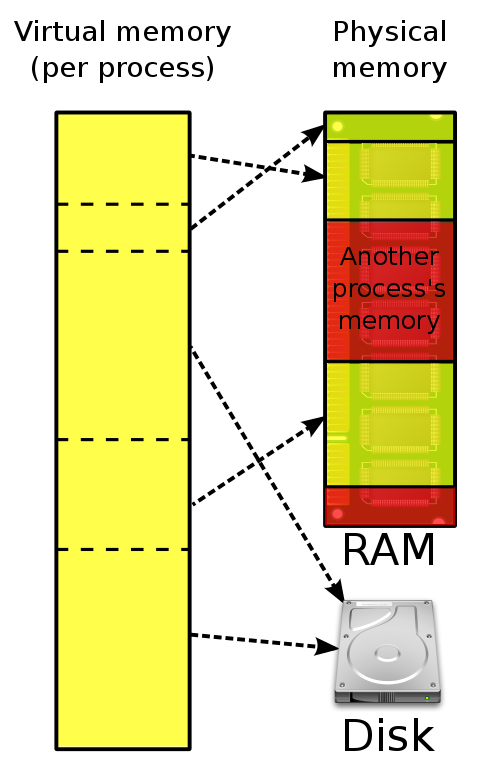
\includegraphics[width=0.9\linewidth]{virtual_memory.png}
        \vspace{-10pt}
        \captionof{figure}{\href{https://en.wikipedia.org/wiki/Virtual_memory}{Virtual Memory. Source: Wikipedia}}
    \end{minipage}

    \vspace{10pt}
    \item \textbf{Expert systems}: Specialized operating systems are created for certain tasks for specific systems. For example, \textbf{real-time systems}, which are specialized systems where the answers have to be given in a maximum time to ensure its correct operation.
\end{itemize}

\subsection{Fourth generation}
The fourth generation of the operating system took place around 1980 and is being used till now. This generation goes hand in hand with personal computers, which already have processors that contain thousands of transistors and are starting to get cheaper.

\begin{itemize}

    \item \textbf{Local Area Network (LAN)}: At the beginning of the 1980s, the first commercial networks for the transfer of information began to be created, so the operating systems must allow the use of these networks. Thanks to this, today we can browse the Internet as we do and we can send and receive information from other computers.

    \begin{minipage}{0.6\linewidth}
        \item \textbf{Distributed computing}: Distributed systems are groups of networked computers which share a common goal for their work.

        In distributed computing, each processor has its own private memory (distributed memory). Information is exchanged by passing messages between the processors. Each computer has its own local memory, and information can be exchanged only by passing messages from one node to another by using the available communication links
    \end{minipage}
    \hfill
    \begin{minipage}{0.34\linewidth}
        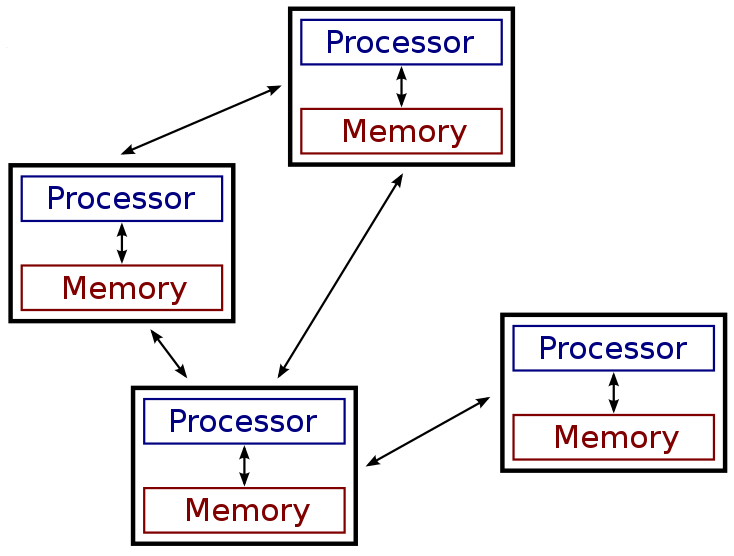
\includegraphics[width=0.9\linewidth]{distributed.png}
        \vspace{-10pt}
        \captionof{figure}{\href{https://en.wikipedia.org/wiki/Distributed_computing\#Parallel_and_distributed_computing}{Source: Wikipedia}}
    \end{minipage}
\end{itemize}



\section{Components}

Each operating system is different, but we can say that the basic components are the same for all of them. The most important components that we are going to study are the following:

\begin{center}
    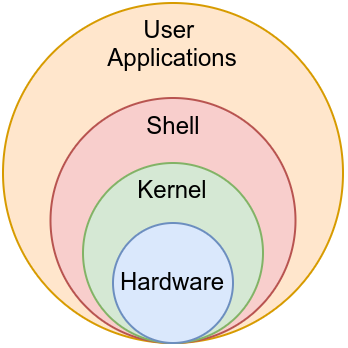
\includegraphics[width=0.4\linewidth]{jerarquia.png}
    \vspace{-10pt}
    \captionof{figure}{Operating System's componentes}
\end{center}



\subsection{Kernel}
The kernel is the central part of the operating system and is responsible for carrying out all the secure communication between the rest of the software and the hardware of the computer.

\vspace{-10pt}
\begin{center}
    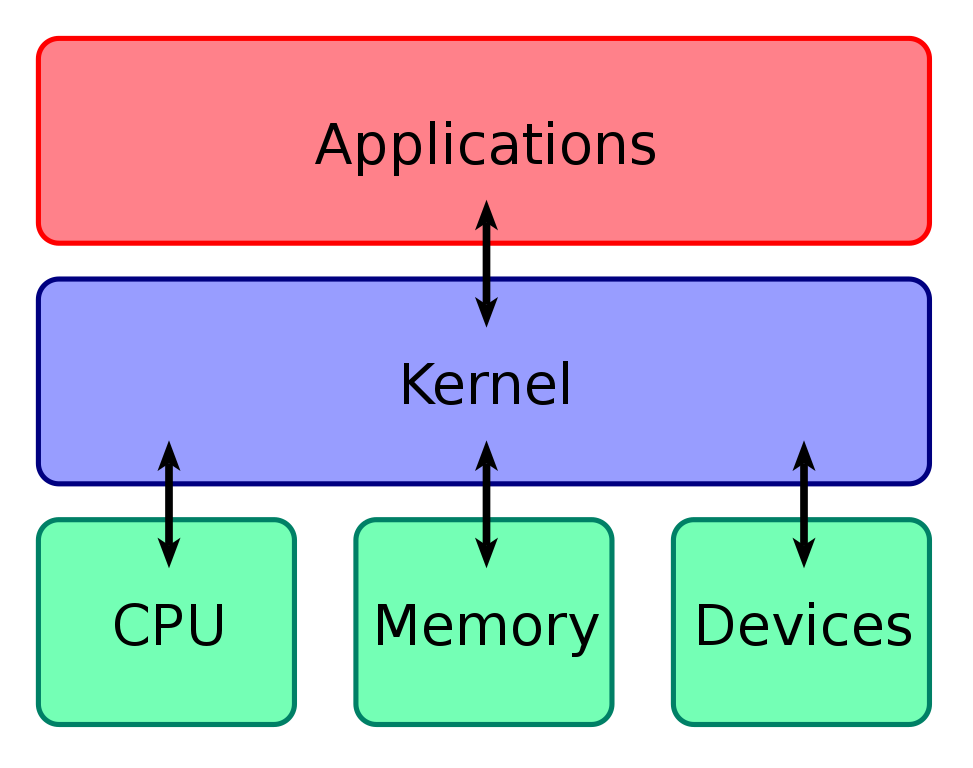
\includegraphics[width=0.5\linewidth]{kernel.png}
    \vspace{-10pt}
    \captionof{figure}{\href{https://en.wikipedia.org/wiki/File:Kernel_Layout.svg}{The kernel connects the applications to the hardware. Source: Wikipedia}}
\end{center}


On most systems, the kernel is one of the first programs loaded on startup (after the bootloader). It handles the rest of startup as well as the CPU,  memory, peripherals, and input/output (I/O).


\subsubsection{Design}

There are different kernel architecture designs.

\begin{itemize}
    \item \textbf{Monolithic kernel}: The first structure used by operating systems was the monolithic one, where is used a single-process kernel. The operating system could only execute one task at a time, composed of a set of interlocking routines in such a way that each one can call any other.

    This is the traditional design of \href{https://en.wikipedia.org/wiki/Unix}{\textbf{Unix}} systems. A monolithic kernel is one single program that contains all of the code necessary to perform every kernel-related task.

    The \textbf{\href{https://en.wikipedia.org/wiki/Linux_kernel}{Linux}} kernel is one of the most representative of this design.

    \item \textbf{Micro-kernels}: Describes an approach to operating system design by which the functionality of the system is moved out of the traditional "kernel", into a set of "servers" that communicate through a "minimal" kernel.

    Most micro-kernels use a message passing system to handle requests from one server to another. They are part of the operating systems like \href{https://en.wikipedia.org/wiki/GNU_Hurd}{\textbf{GNU Hurd}} and \href{https://en.wikipedia.org/wiki/Minix}{\textbf{MINIX}}.

    \item \textbf{Hybrid (or modular) kernels}: hey are similar to micro kernels, except they include some additional code in kernel-space to increase performance. These kernels represent a compromise that was implemented by some developers to accommodate the major advantages of both monolithic and micro kernels.

    Hybrid kernels are used in most commercial operating systems, such as Microsoft Windows 10 and Apple's own macOS.

    \item \textbf{In layers or levels}: The design of these operating systems is built on top of the hardware in virtual overlapping levels until reaching the end user level. Designed for \href{https://en.wikipedia.org/wiki/THE_multiprogramming_system}{THE operating system} in 1968 by E. W. Dijkstra's team.
    \begin{itemize}
        \item \textbf{Level 0}: The hardware.
        \item \textbf{Level 1}: The CPU management.
        \item \textbf{Level 2}: The memory management, which allow to allocate memory to processes.
        \item \textbf{Level 3}: Dealt with communication between the operating system and the system console..
        \item \textbf{Level 4}: Managed all I/O between the devices attached to the computer.
        \item \textbf{Level 5}: Consisted of user programs.
    \end{itemize}


    \begin{center}
        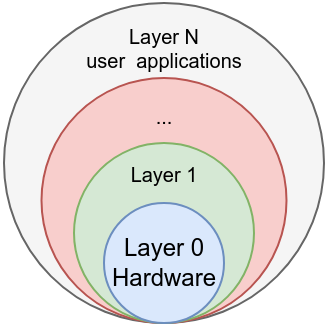
\includegraphics[width=0.5\linewidth]{layered.png}
    \end{center}
\end{itemize}

An operating system is a very complex program, so even if its main design is one of those previously mentioned, it is most likely that it will also make use of other designs as far as possible.

For example, Linux is a monolithic kernel, but it also has the option to load/unload drivers (it's modular too).


\subsection{Shell}
The “\textbf{shell}”, in operating systems, is the computer program that exposes an operating system's services to a human user or other programs.

In general, operating system shells use either a command-line interface (\textbf{CLI}) or graphical user interface (\textbf{GUI}).



\begin{mycode}{\textbf{BASH} command line interface (CLI) in GNU/Linux}{console}{}
ruben@vega:/etc/etckeeper $ ls -lh

total 48K
drwxr-xr-x 2 root root 4,0K abr 13 09:36 commit.d
-rwxr-xr-x 1 root root  551 oct 28  2019 daily
-rw-r--r-- 1 root root 1,5K oct 28  2019 etckeeper.conf
drwxr-xr-x 2 root root 4,0K abr 13 09:36 init.d
drwxr-xr-x 2 root root 4,0K abr 13 09:36 list-installed.d
drwxr-xr-x 2 root root 4,0K abr 13 09:36 post-install.d
drwxr-xr-x 2 root root 4,0K abr 13 09:36 pre-commit.d
drwxr-xr-x 2 root root 4,0K abr 13 09:36 pre-install.d
drwxr-xr-x 2 root root 4,0K abr 13 09:36 unclean.d
drwxr-xr-x 2 root root 4,0K abr 13 09:36 uninit.d
drwxr-xr-x 2 root root 4,0K abr 13 09:36 update-ignore.d
drwxr-xr-x 2 root root 4,0K abr 13 09:36 vcs.d

\end{mycode}


\section{Operating system's functions}
The main function of the operating system is to manage the hardware resources of the computer and allow the execution of user programs. To do this, it must perform various functions.

\begin{itemize}
    \item Process management
    \item RAM memory management
    \item Input/Output management
    \item File management
    \item Networking
    \item Security
\end{itemize}

We will see each of these functionalities in the following chapters.






\section{How operating systems works}

In a simplified way, an operating system works as follows:

\begin{center}
    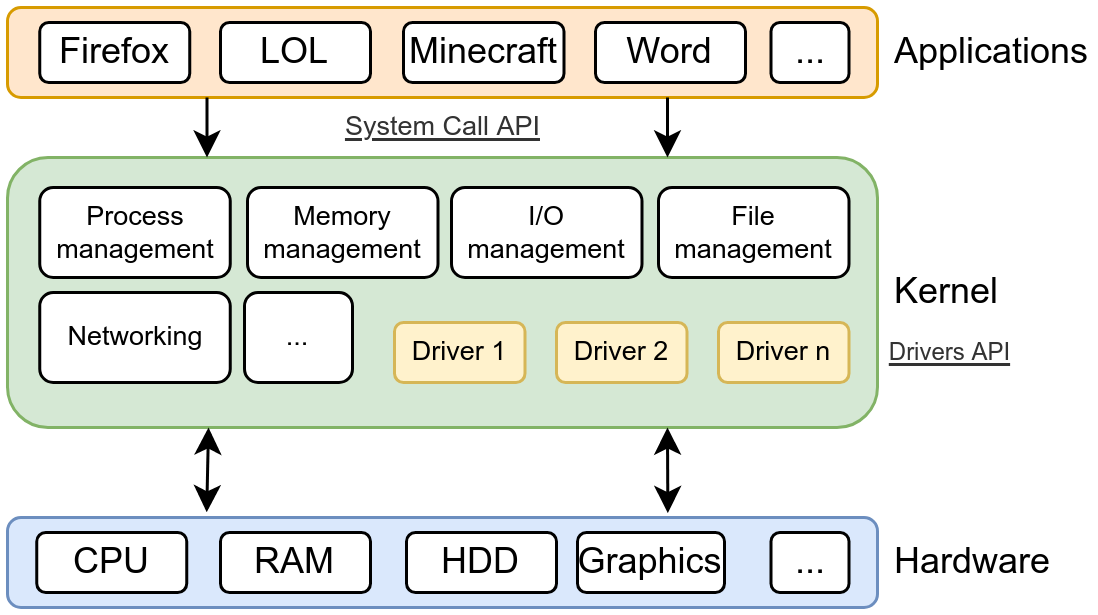
\includegraphics[width=0.75\linewidth]{how_works.png}
\end{center}





\chapter{Process management}
A process is a program in execution. The OS must allocate resources to processes, enable processes to share and exchange information, protect the resources of each process from other processes and enable synchronization among processes.







\chapter{RAM memory management}



\chapter{Input/Output management}


\chapter{File management}


\chapter{Networking}


\chapter{Security}